\documentclass[8pt, twocolumn]{article}
\usepackage{graphicx}

\title{Assignment 1}
\author{Sahishnu, CS21BTECH11009}
\date{}

\begin{document}

\maketitle
\textbf {2.(c)}\\
\begin{center}
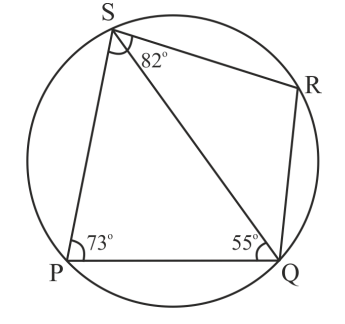
\includegraphics[scale=0.5]{figs/fig1.png}

\end{center}
PQRS is a cyclic quadrilateral. Given \angle $QPS=73^o$, \angle $PQS=55^o$ and \angle $PSR=82^o$, calculate:\\
(i) \angle $QRS$\\
(ii) \angle $RQS$\\
(iii) \angle $PRQ$\\\\
\textbf {Solution: }\\\\
(i) We know that, In a Cyclic quadrilateral, sum of a pair of opposite angles results in $180^o$.
Hence,
\begin{center}
   $\angle QPS + \angle QRS = 180^o$
\end{center}
\begin{center}
$\rightarrow 73^o + \angle QRS = 180^o$
\end{center}
\begin{equation}
    \Rightarrow \angle QRS = 107^o
\end{equation}
(ii) Again, from the fact that sum of a pair of opposite angles is $180^o$,
\begin{center}
    $\angle PSR + \angle PQR = 180^o$
\end{center}
\begin{center}
    $\rightarrow 82^o + \angle PQS + \angle RQS = 180^o $
\end{center}
\begin{center}
    $\rightarrow 82^o + 55^o + \angle RQS = 180^o$
\end{center}
\begin{equation}
    \Rightarrow \angle RQS = 43^O
\end{equation}
(iii) We know that in a circle, a chord always subtends equal angles at all the points on a particular arc. Consider the chord "PQ",
\begin{equation}
    \rightarrow \angle PSQ = \angle PRQ
\end{equation}
We know that the sum of angles in a triangle equals to $180^o$, Consider the triangle $\triangle PQS$,
\begin{center}
    $\rightarrow \angle PSQ + \angle SPQ + \angle PQS = 180^o$ 
\end{center}
\begin{center}
    $\rightarrow \angle PSQ + 73^o + 55^o = 180^o $
\end{center}
\begin{center}
    $\rightarrow \angle PSQ = 52^o$
\end{center}
Substituting this result in the equation (3),
\begin{equation}
    \Rightarrow \angle PRQ = 52^o
\end{equation}
\end{document}
